\documentclass[tikz,border=8pt]{standalone}
\usetikzlibrary{arrows.meta,positioning}
\begin{document}
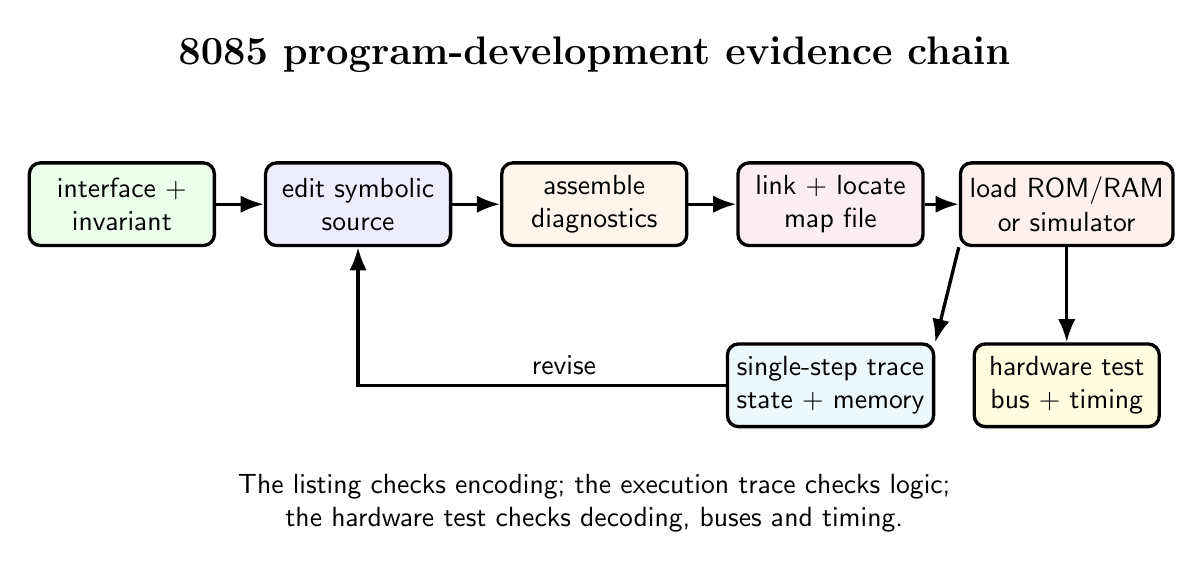
\begin{tikzpicture}[font=\sffamily,>=Latex,
 phase/.style={draw,very thick,rounded corners,minimum width=2.35cm,minimum height=1.05cm,align=center}]
\node[font=\Large\bfseries] at (7.25,5.45) {8085 program-development evidence chain};
\node[phase,fill=green!8] (spec) at (1.25,3.55) {interface +\\invariant};
\node[phase,fill=blue!7] (edit) at (4.25,3.55) {edit symbolic\\source};
\node[phase,fill=orange!8] (asm) at (7.25,3.55) {assemble\\diagnostics};
\node[phase,fill=purple!7] (link) at (10.25,3.55) {link + locate\\map file};
\node[phase,fill=red!6] (load) at (13.25,3.55) {load ROM/RAM\\or simulator};
\foreach \a/\b in {spec/edit,edit/asm,asm/link,link/load}{\draw[very thick,->] (\a)--(\b);}
\node[phase,fill=cyan!8] (trace) at (10.25,1.25) {single-step trace\\state + memory};
\node[phase,fill=yellow!12] (hard) at (13.25,1.25) {hardware test\\bus + timing};
\draw[very thick,->] (load)--(hard);
\draw[very thick,->] (load.south west)--(trace.north east);
\draw[very thick,->] (trace.west) -| node[pos=.22,above] {revise} (edit.south);
\node[align=center] at (7.25,-.25) {The listing checks encoding; the execution trace checks logic;\\the hardware test checks decoding, buses and timing.};
\end{tikzpicture}
\end{document}
